\documentclass[12pt]{article}
\usepackage{fullpage,url,amssymb,epsfig,color,xspace,tikz,amsmath, amsthm}
\usetikzlibrary{calc,shapes.multipart,chains,arrows}
\usepackage{graphicx}
\begin{document}

\begin{center}
    \textbf{\huge Tutorial 3}
\end{center}

\section{pointers}
\begin{itemize}
    \item What is a pointer?
    %pointer stores the address that it points to.
    \item Why do we use pointers?
    \item What is the output?
    \begin{verbatim}
#include <iostream>
using namespace std;

struct Coord {
  int x;
  int y;
};

int main() {
  int a = 0;
  int b = 1;
  int *p1 = &b;
  int *p2 = &a;
  p1 = &a;
  *p1 = 10;
  int **p3 = &p2;
  p2 = *&*&p1;
  Coord *c = new Coord{*p2, **p3};
  **p3 = 4;
  *p3 = p1;
  c->y = **p3;
  **p3 = 8;
  cout << *p1 << ' ' << *p2 << ' ' << **p3 << endl;
  cout << c->x << ' ' << c->y << endl;
  delete c;
}
    \end{verbatim}
\end{itemize}

\section{Linked List}

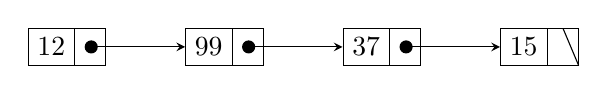
\begin{tikzpicture}[list/.style={rectangle split, rectangle split parts=2,
    draw, rectangle split horizontal}, >=stealth, start chain]

  \node[list,on chain] (A) {12};
  \node[list,on chain] (B) {99};
  \node[list,on chain] (C) {37};
  \node[list,on chain] (D) {15};
  %\draw (D.north east) -- (D.south west);
  \draw (D.two north) -- (D.south east);
  \draw[*->] let \p1 = (A.two), \p2 = (A.center) in (\x1,\y2) -- (B);
  \draw[*->] let \p1 = (B.two), \p2 = (B.center) in (\x1,\y2) -- (C);
  \draw[*->] let \p1 = (C.two), \p2 = (C.center) in (\x1,\y2) -- (D);
\end{tikzpicture}

\begin{verbatim}
struct Node {
    string/int val;
    Node *next;
};
\end{verbatim}

\subsection{Exercise}
\begin{enumerate}
    \item Implement queue using linked list
    \begin{verbatim}
struct Node {
    int val;
    Node *next;
};
struct Queue {
    Node *frt;
    Node *last;
};

Queue *initQueue(); //initialize an empty Queue
bool isEmpty(Queue *q); //check if a queue is empty
void add(Queue *q, int val); //add an element to the back of a queue
void remove(Queue *q); //remove an element form the front of a queue
bool check(Queue *q, int num); //check if an element is in the queue
void nuke(Queue *q); //delete all elements in the queue
    \end{verbatim}
    \item Now implement queue using vector
\end{enumerate}

\end{document}